\documentclass{article}

\usepackage{upgreek}
\usepackage{amsmath}
\usepackage{minted}
\usepackage{graphicx}
\usepackage{caption}
\usepackage{subcaption}
\usepackage{mathrsfs}
\usepackage[toc,page]{appendix}

%Section style
\usepackage{etoolbox} %for configuration of sloppy
\usepackage{xcolor}


\definecolor{secnum}{RGB}{102,102,102}

\makeatletter
    \def\@seccntformat#1{\llap{\color{secnum}\csname the#1\endcsname\hskip 16pt}}
\makeatother
%end section style

\begin{document}

\section{II.1}

\subsection{II.1.1}

We implemented the LDA ourselves. The code can be seen in
Part1/Opgavei11.m. 

On the training data we observe a 14.00 \% miss rate while on the test data
the rate is 21.05 \%.

\subsection{II.1.2}

After normalizing the data we observed the same error as on the
non-transformed data. 

This is unsurprising as normalization preserves the relation inbetween
the elements of the dataset. Graphically a plot of the data set would
look identical except for a change of the axises. Finally LDA uses the
covariance which fully describes the distribution of the data and thus
renders normalization redundant.

\subsection{II.1.3}

Muh Bayes.


\subsection{II.2.1}

We used the linear model
\begin{equation}
    y(x, w) = w_0 + w_1 x_1 + ... + w_D x_D
\end{equation}
and calculated the RMS using the python library sklearn. this gave us the fittings seen on 
figure \ref{fig:II21}. It seams Selection 2 provides the best prediction, but giving the problem some though, we concluded it mearly copies
the previous years sunspot numbers. So even if it does have the lowest RMS, it is not guarantede to be the best model.

\begin{figure}[!ht]
    \centering
    \begin{subfigure}[b]{0.5\textwidth}
        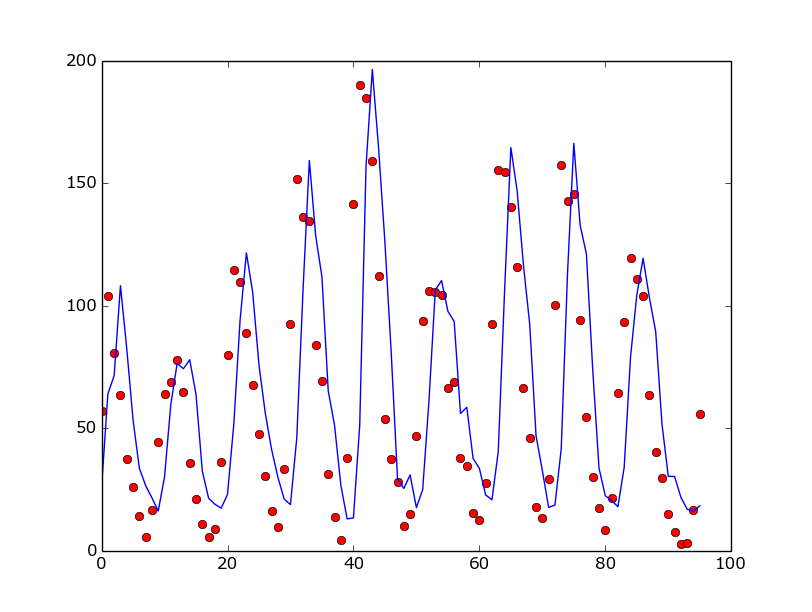
\includegraphics[width=\textwidth]{Part2/II211.png}
        \caption{fitting with $RMS = 64.4180$}
    \end{subfigure}%
    \begin{subfigure}[b]{0.5\textwidth}
        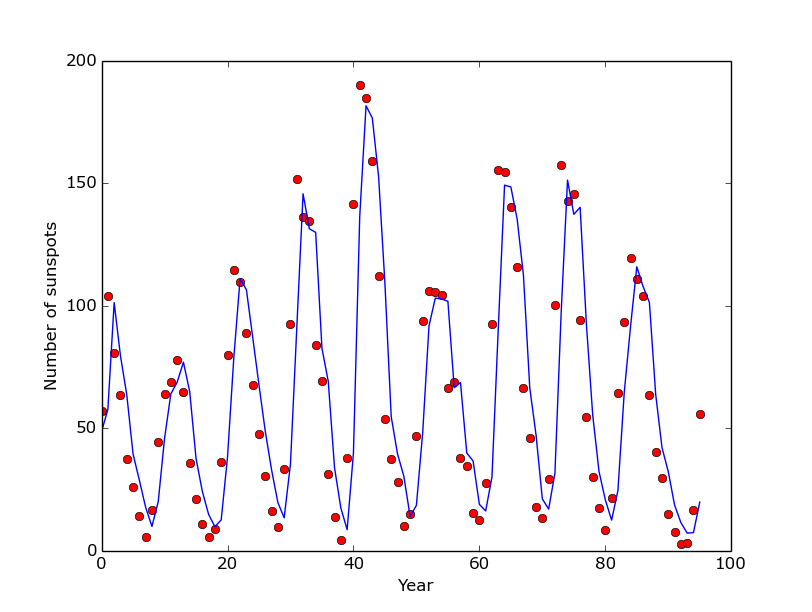
\includegraphics[width=\textwidth]{Part2/II212.png}
        \caption{fitting with $RMS = 30.1460$}
    \end{subfigure}
    \begin{subfigure}[b]{0.5\textwidth}
        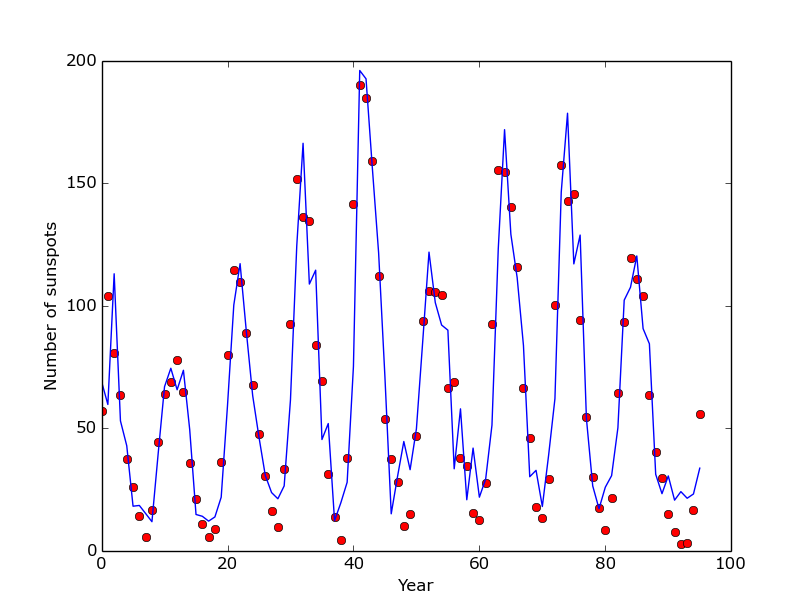
\includegraphics[width=\textwidth]{Part2/II213.png}
        \caption{fitting with $RMS = 49.8736$}
    \end{subfigure}
    \caption{Fittings using linear regression and ML}
    \label{fig:II21}
\end{figure}


\subsection{II.2.2}

We used the following to calculate our maximum posterior weight vector.\\
\begin{align*}
    % p(w|\alpha) &= \mathcal{N}(w|0, \alpha^{-1}\textbf{I})\\
    m_{N} &= \beta S_{N} \Phi^{T} \textbf{t}\\
    S_{N} &= (\alpha \textbf{I} \cdot \beta \Phi^{T} \Phi)^{-1}
\end{align*}
We also know $w_{MAP} = m_N$.\\
Giving the constant variable $\beta = 1$ we can reduce the equations to the following\\
\begin{align*}
    w_{MAP} &= (\alpha \textbf{I} \cdot \Phi)^{-1} \textbf{t}
\end{align*}

\subsection{II.2.3}

I dont like crying

\end{document}
